\newpage

\section{Обзор базовых инструментов}
\subsection{Материалы}
Давайте попробуем создать наш первый материал, задать ему цветовой параметр, а 
также посмотрим как динамически менять данный параметр.

Но сначала дадим определение материалу. \textbf{Материал} в ue - это
специальный вид ассета, который отвечает за визуальную часть, как будет
выглядеть статический меш, скелетал меш, системы частиц. Это шейдер, подпрограмма, 
работающая на GPU, которая вычисляет цвета, положение пикселей на сцене.

Для того, чтобы создать материал, кликаем правой кнопкой мыши в 
\textbf{Content Browser}'е и в сплывающем окне выбираем ассет \textbf{Material}.
Нейминг у материала следующий: \textbf{M\_NameOfMaterial}. Кликаем по созданному нами 
материалу, после чего открывается редактор материала - это специализированный
редактор, который отвечает за обработку параметров материала.

Для того, чтобы установить цвет материалу достаточно подсоединить к входу BaseColor
материала вектор с 4 параметрами: \textbf{кликаем правой кнопкой мыши по свободной
области -> ищем Constant4Vector -> и подсоединяем этот вектор к BaseColor}.
Теперь, если мы кликнем по добавленной ноде, в панеле Details мы сможем
настроить цвет нашему материалу, назначив значения R, G, B, A параметрам либо
через Color Picker.

\begin{figure}[h]
    \centering
    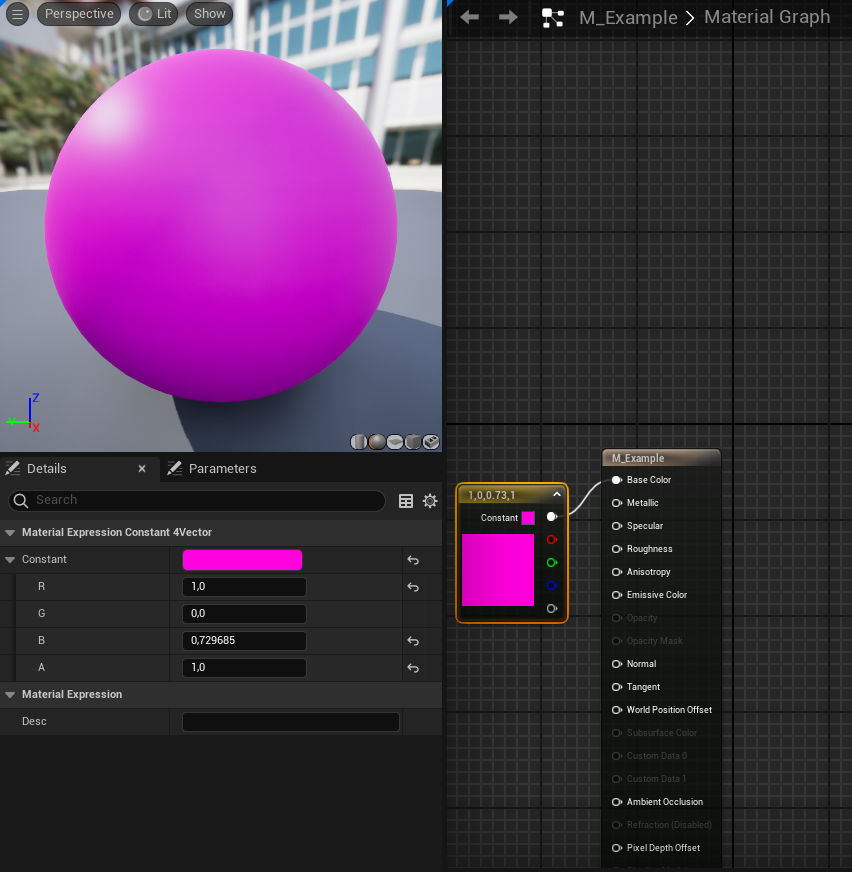
\includegraphics[width=\textwidth]{Lections/Lection_2/BaseColorMaterial.png}
    \caption{Установка цвета материалу}
\end{figure}

\subsubsection*{Горячие клавиши:}

1.\hspace{1em}1->Левая кнопка мыши - константа с 1 значением.

2.\hspace{1em}2->Левая кнопка мыши - константа с 2 значениями.

3.\hspace{1em}3->Левая кнопка мыши - константа с 3 значениями.

4.\hspace{1em}4->Левая кнопка мыши - константа с 4 значениями.


Мы уже можем пользоваться нашим материалом. Для этого достаточно drag-and-drop'ом 
перетащить его на какой-либо объект на сцене, либо установив его в панеле
Details данного объекта в категории Materials.

Давайте превратим наш цвет в параметр - для этого: \textbf{кликаем правой кнопкой 
мыши по ноде цвета -> в сплывающем окне выбираем ConvertToParametr}.

Теепрь создадим другой вид ассета материала - \textbf{Material Instance}. 
Для этого: \textbf{кликаем правой кнопкой мыши по материалу в Content Browser'е 
-> в сплывающем окне выбираем Create Material Instance}. 
Нейминг у экземпляра материала следующий: \textbf{MI\_NameOfMaterialInstance}.

Зачем разделять Material и Material Instance?

\textbf{Material} - это базовый шаблон, содержащий все основные настройки и 
вычисления, которые определяют внешний вид. Материал создаётся как основной 
и описывает весь шейдерный код, который будет использоваться для его рендеринга.

\textbf{Material Instance (Экземпляр материала)} - экземпляр материала представляет 
собой более производительную и гибкую версию основного материала. 
Он создаётся на основе уже существующего Material и позволяет менять его параметры
без необходимости компиляции нового шейдера.
Material Instances обеспечивают более быстрые изменения и низкую нагрузку на GPU,
поскольку они используют уже скомпилированные настройки шейдера из основного 
материала.

В нашем случае у нашего экземпляра метериала всего один параметр - его цвет,
который мы создали в редакторе материала. Мы можем установить новый цвет. Далее
мы также можем создать новый экземпляр материала и поставить ему другой цвет.

\begin{figure}[h]
    \centering
    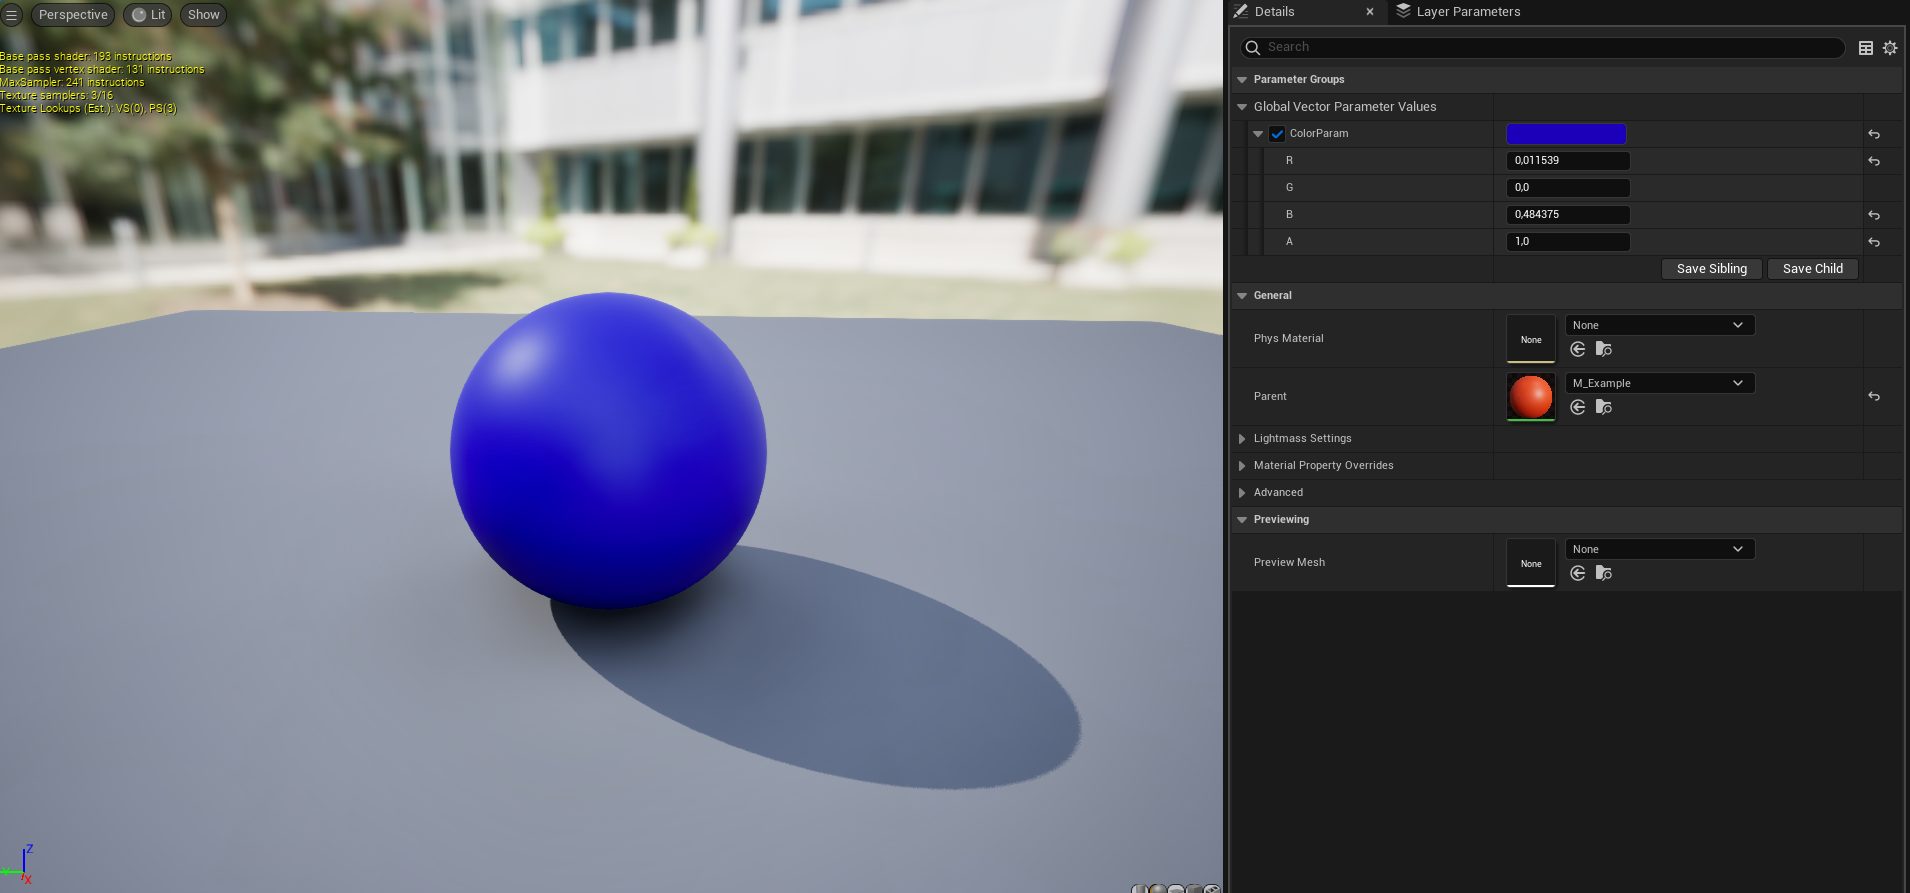
\includegraphics[width=\textwidth]{Lections/Lection_2/MaterailInst.png}
    \caption{Установка цвета экземпляру материала}
\end{figure}

Таким образом, мы можем насоздавать кучу экземпляров с различными цветами.
Но такой способ иемеет значительный минус - для каждого цвета придётся 
создавать отдельный экземпляр, который будет занимать какое-то количество памяти
на диске. Лучшим способ будет динамическое создание экзмепляров материала.

У StaticMeshComponent'а есть метод \textbf{Create Dynamic Material Instance},
который создаёт копию указанного материала или его экземпляра, давая возможность 
модифицировать её свойства прямо во время игры. Это важно, так как статические 
Material Instances, созданные через редактор, не позволяют менять параметры на лету.
И данный метод вернёт нам ссылку на созднанный \textbf{Material Instance Dynamic}.

И этому \textbf{Material Instance Dynamic} мы можем с помощью метода \textbf{
Set Vector Parameter Value} установить нашему параметру новое значение. 
Методу надо передать имя параметра, которое мы создали в материале, и 
само новое значение.

\begin{figure}[h]
    \centering
    \includegraphics[width=\textwidth]{Lections/Lection_2/CreatedynamicMat.png}
    \caption{Создание динамического экземпляра материала}
\end{figure}

\subsection{Динамическое создание AActor}

Функция для спавна AActor называется \textbf{Spawn Actor from Class}.

\subsubsection*{Какие аргументы имеет эта функция?:}

1.\hspace{1em}Class - здесь мы должны выбрать класс AActor, который мы хотим
заспавнить.

2.\hspace{1em}SpawnTransform - аргумент определяет трансформацию создаваемому объекту.

3.\hspace{1em}Collision Handling Override - определяет, как обрабатывать 
столкновения актора при создании. Варианты:

Always Spawn, Ignore Collisions – создает актор, игнорируя любые препятствия.
Adjust Location But Always Spawn – перемещает актор, чтобы избежать коллизий, но 
все равно создает его.
Dont Spawn if Colliding – не создает актор, если в месте спавна есть коллизия.
Try to Adjust Location, But Don't Spawn if Still Colliding – пытается переместить 
актор при коллизии, и если не удается избежать коллизий, актор не создается.

4.\hspace{1em}Instigator - тот объект, который инициировал создание AActor.
Обычно используется в игровых механиках для передачи информации о том, кто 
именно запустил появление AActor (например, для указания персонажа, запустившего 
какой-либо снаряд).

Функция \textbf{Spawn Actor from Class} возвращает ссылку на созданный AActor.
На рисунке 14 приведён пример создания StaticMeshActor'а.
После создания необходимо установить параметры созданному AActor и прежде 
необходимо устновить StaticMeshComponent'у свойство Mobility в Movable с помощью 
метода \textbf{Set Mobility} для того,чтобы можно было в реальном времени 
менять свойства этому компоненту.
Далее устанавливается статическая сетка с помощью метода \textbf{Set Static Mesh}.
Установим, например, Sphere выбрав этот меш в аргументе NewMesh.
Потом мы можем установить материал данному мешу с поомщью метода \textbf{Set 
Material}.

\begin{figure}[h]
    \centering
    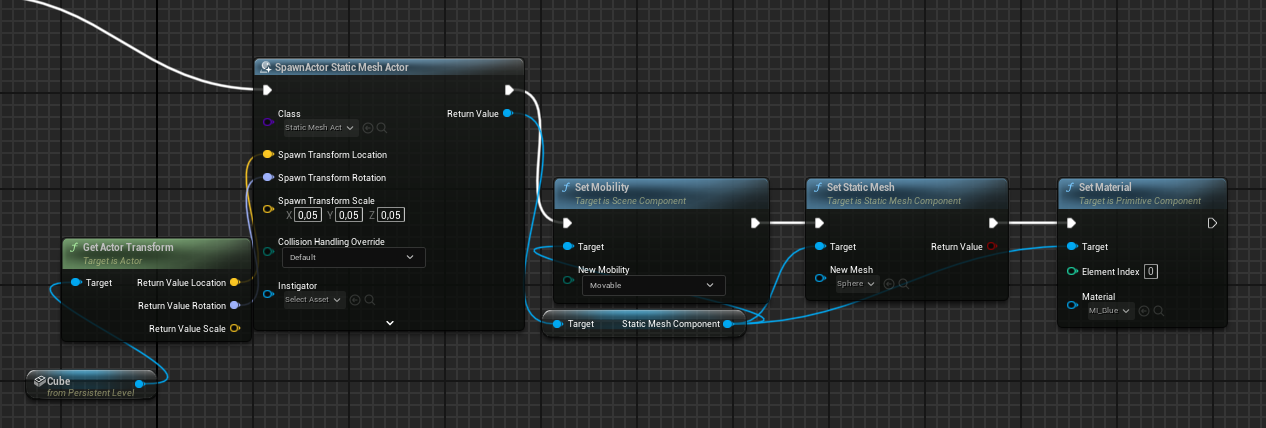
\includegraphics[width=\textwidth]{Lections/Lection_2/SpawnActor.png}
    \caption{Динамическое создание AActor}
\end{figure}

\subsection{Создание первого Blueprint класса, унаследованного от AActor}

Blueprint класс можно создать следующим способом: \textbf{кликаем правой кнопкой 
мыши по свободной области в Content Browser'е -> в сплывающем окне выбираем 
Blueprint Class}. Откроется менюшка, где будет представлен список наиболее
часто используемых классов и компонентов, от которых мы можем унаследоваться.
Стоит понимать, что при наследовании мы берём функционал какого-то объекта и имеем
возможность его расширить. 

\begin{figure}[h]
    \centering
    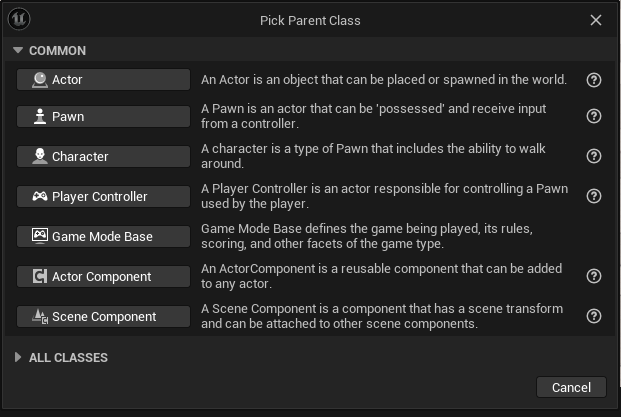
\includegraphics[width=\textwidth]{Lections/Lection_2/CreateBPActor.png}
    \caption{Меню выбора класса, от которого можно унаследоваться}
\end{figure}

Выбираем AActor и даём ему какое-то имя. Нейминг у блупринтов следующий: 
\textbf{BP\_NameOfBlueprint}.

Что мы выидим при открытии редактора блупринтов?

\textbf{Viewport (Видовой экран)} – область, где можно визуально просматривать 
и настраивать компоненты Blueprint'а. Здесь можно изменять их положение, поворот 
и масштаб, чтобы видеть, как они будут выглядеть и взаимодействовать друг с 
другом в игре.

\textbf{Graph (Граф)} – основная рабочая область, где создаются и соединяются ноды 
(узлы) для построения логики. Здесь располагаются все ноды: переменные, функции, 
события и прочие элементы, которые визуально соединяются линиями. 
Граф отображает всю логику вашего Blueprint'а. Вы с этим занимались на прошлом уроке
и в домашнем задании.

\textbf{My Blueprint (Мой Blueprint)} – панель слева, где находятся переменные, 
функции, макросы, события и графы, доступные для текущего Blueprint'а. 
Через эту панель можно добавлять новые переменные, функции и даже дополнительные 
графы для организации сложной логики. Это также центральное место для управления 
структурой и содержанием вашего Blueprint'а.

\textbf{Details (Сведения)} – правая панель, которая отображает свойства и 
настройки выбранного элемента. Здесь можно 
настроить поведение конкретного узла или изменить свойства, такие как значение 
переменной, настройки функций, а также параметры компонентов.

\textbf{Components (Компоненты)} – панель, которая позволяет добавлять физические 
и визуальные элементы, такие как Static Mesh или Skeletal Mesh, к вашему 
Blueprint'у. Например, если вы работаете с Blueprint'ом для персонажа, здесь 
можно добавлять и настраивать руки, голову, камеру и т.д. Компоненты служат 
основой для визуальной и физической структуры актора.

\textbf{Toolbar (Панель инструментов)} – верхняя панель, которая предоставляет доступ к 
основным функциям, таким как компиляция Blueprint'а, проверка его ошибок и 
запуск симуляции. Здесь же находятся кнопки для сохранения, настройки и 
перехода к родительскому Blueprint'у.

\textbf{Construction Script} – это специальный граф, предназначенный для выполнения
логики во время создания или обновления объекта прямо в редакторе. Этот скрипт 
автоматически запускается каждый раз, когда объект перемещается, изменяется или 
когда его параметры обновляются. Он помогает настраивать объект ещё до начала игры,
предоставляя возможность увидеть результаты изменений сразу в редакторе.

\subsubsection*{Основные особенности Construction Script:}

a.\hspace{1em}Исполнение при изменениях – Construction Script выполняется при 
любом изменении актора в редакторе. Например, если вы перемещаете объект или 
меняете его свойство, Construction Script тут же обновляет его. Это удобно для 
настройки и визуального тестирования объектов.

b.\hspace{1em}Выполнение кода только в редакторе – код в Construction Script 
выполняется только в редакторе, а не в игровом процессе. Поэтому он не влияет на 
производительность игры, а используется лишь для подготовки объектов.